\documentclass[11pt]{article}
\usepackage[a4paper,margin=1in]{geometry}
\usepackage{graphicx}
\usepackage{float}
\usepackage{caption}
\usepackage{hyperref}
\usepackage{amsmath}
\usepackage{booktabs}
\usepackage{enumitem}

\graphicspath{{artifacts/plots/}}

\title{Vuvuzela Noise Reduction Report}
\author{}
\date{}

\begin{document}
\maketitle

\section{How the filter design specifications were chosen}

I chose the specifications from direct signal inspection and the delay constraint.

First, I compared the noisy commentary and the vuvuzela reference in the time domain. The interference appears quasi-periodic rather than broadband, which indicates tonal/harmonic noise and motivates harmonic suppression instead of a single wide stopband.

\begin{figure}[H]
    \centering
    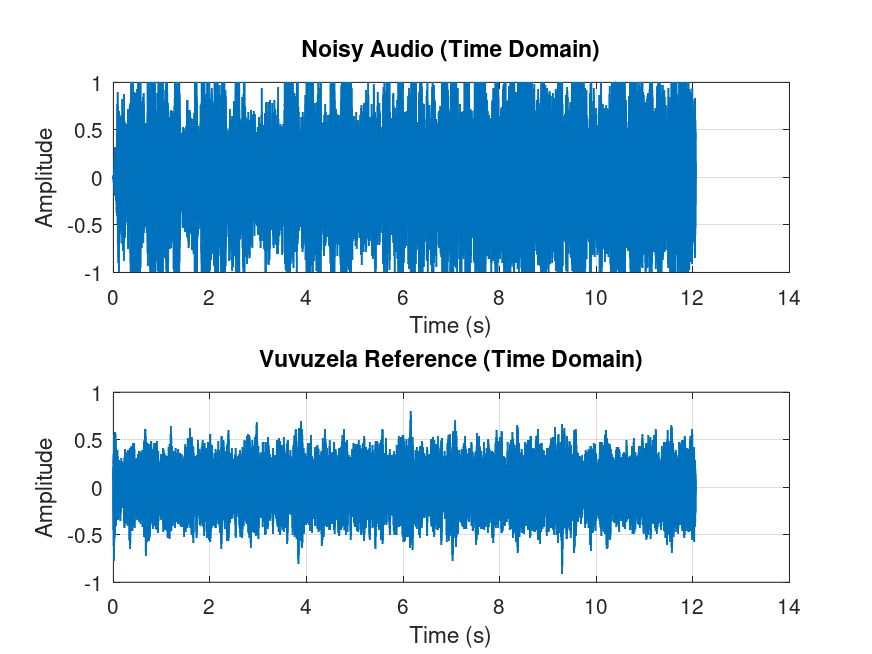
\includegraphics[width=0.84\linewidth]{mat_01_time_domain_inputs.png}
    \caption{Time-domain comparison used to identify tonal interference.}
\end{figure}

Second, I examined the vuvuzela PSD and estimated a fundamental near 235 Hz with regularly spaced harmonics. This led to harmonic-centered attenuation bands (with finite bandwidth) rather than single-bin cancellation.

\begin{figure}[H]
    \centering
    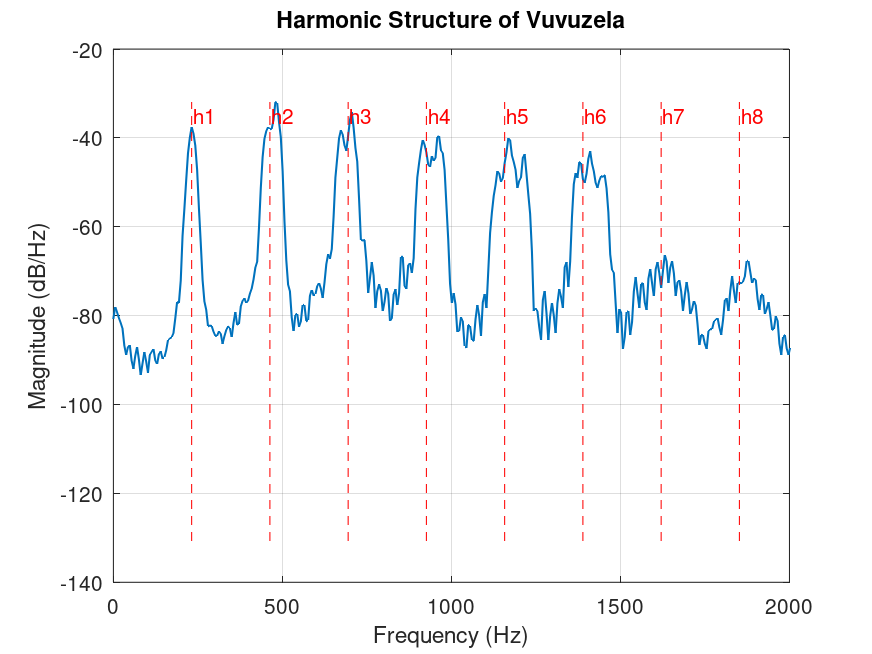
\includegraphics[width=0.84\linewidth]{mat_02_vuv_harmonic_structure.png}
    \caption{Harmonic structure used to set harmonic suppression targets.}
\end{figure}

Third, I compared noisy and reference PSDs to separate speech-dominant and interference-dominant regions. This supported preserving the speech band and suppressing harmonic regions.

\begin{figure}[H]
    \centering
    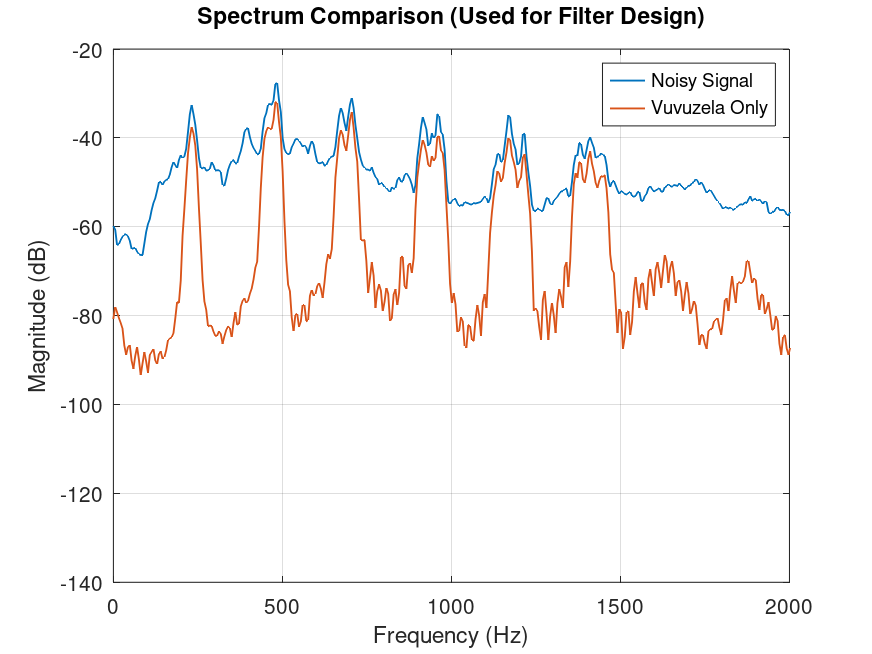
\includegraphics[width=0.84\linewidth]{mat_03_spectrum_design_comparison.png}
    \caption{PSD comparison used for passband/stopband decisions.}
\end{figure}

Finally, I selected STFT parameters that satisfy delay while giving enough frequency resolution: $N_{FFT}=1024$, hop $=256$ (75\% overlap) at $f_s=8$ kHz. This gives a 128 ms frame and 32 ms hop, with effective frame-center delay about 64 ms, which is within the 0.2 s requirement.

\section{Design specifications}

The implemented specifications are:
\begin{itemize}
    \item \textbf{Speech passband target:} 300--3400 Hz.
    \item \textbf{Low-frequency suppression:} below 180 Hz to reduce rumble.
    \item \textbf{Harmonic stop-regions:} around $h_k=kf_0$, $k=1..8$, with $f_0\approx235$ Hz and mask bandwidth 56 Hz.
    \item \textbf{STFT length:} 1024 samples, hop 256 (75\% overlap).
    \item \textbf{Adaptive gains:} Wiener + spectral subtraction with $\alpha=1.35$, oversubtraction $=1.25$, gain floor $=0.03$.
    \item \textbf{Notch specification:} second-order IIR notches with $Q=22$ at each $h_k$ and $h_k\pm12$ Hz.
    \item \textbf{Polishing filters:} second-order Butterworth high-pass (140 Hz), bandpass (900--3400 Hz), and low-pass (2000 Hz).
\end{itemize}

Target behavior was strong harmonic attenuation with controlled speech loss; achieved proxy values were approximately speech change $-6.58$ dB and harmonic-band change $-24.82$ dB.

\section{Filters designed, frequency response, and obtained orders}

I designed a hybrid filter bank with one adaptive stage and fixed IIR sections:
\begin{enumerate}
    \item \textbf{Adaptive STFT filter} (Wiener + spectral subtraction + harmonic masking): time-varying, so no single fixed order.
    \item \textbf{Notch cascade:} 24 second-order IIR notches (8 harmonics, each with center and $\pm12$ Hz companions), $Q=22$.
    \item \textbf{Butterworth shaping filters:} second-order high-pass (140 Hz), second-order bandpass (900--3400 Hz), second-order low-pass (2000 Hz), plus a small second-order intelligibility bandpass (1400--2200 Hz).
\end{enumerate}

Figure 4 shows magnitude and phase responses. The notch panel overlays all notch sections and confirms deep narrow attenuation around harmonic families. The Butterworth panels show smooth spectral shaping for speech preservation and rumble/high-frequency control. Although individual IIR sections have nonlinear phase, forward-backward filtering is used in implementation to remove net phase distortion in the output.

\begin{figure}[H]
    \centering
    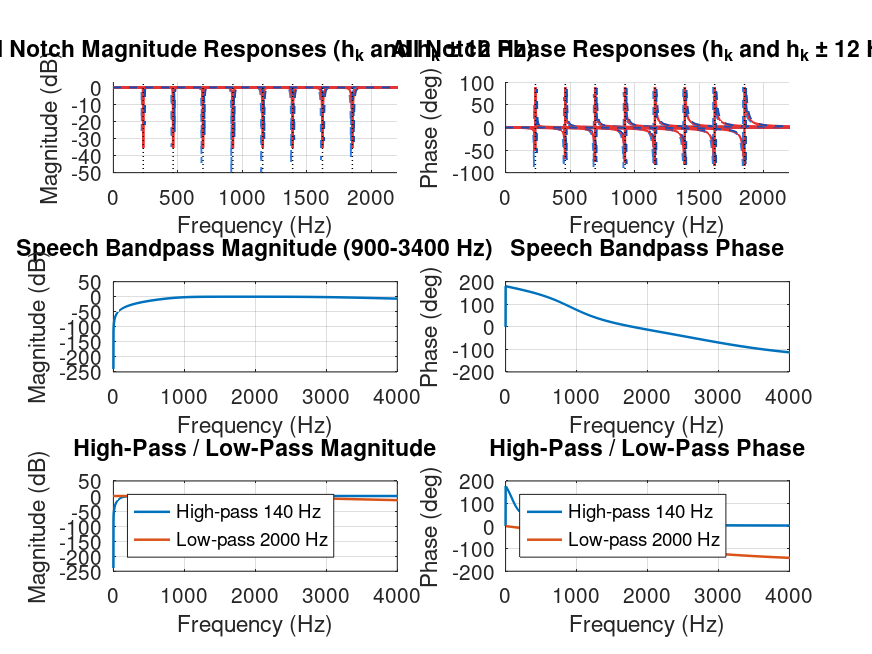
\includegraphics[width=0.9\linewidth]{mat_08_filter_responses_mag_phase.png}
    \caption{Magnitude and phase responses of the designed notch bank and Butterworth sections.}
\end{figure}

\textbf{Obtained orders:} notches are second-order each (24 sections total), and each Butterworth stage is second-order. The adaptive STFT stage is time-varying and therefore has no fixed classical LTI order.

\section{Tradeoffs and limitations}

The main tradeoff was suppression strength versus speech naturalness. Stronger harmonic masking and post-gating reduce buzzing more, but can create hollow or metallic speech. I tuned parameters to keep speech intelligible while strongly reducing harmonic peaks.

A second tradeoff was frequency resolution versus delay. Longer frames improve harmonic separation but increase latency. The chosen 1024-sample frame gives adequate harmonic resolution while keeping delay comfortably under 0.2 s.

The method also has limitations: it assumes a relatively stable harmonic interference pattern and uses non-causal forward-backward filtering (offline processing). In addition, no clean speech reference is available, so evaluation relies on proxy spectral metrics and listening tests rather than ground-truth SNR/quality scores.

Overall, the approach meets the goal: substantial harmonic suppression with preserved speech intelligibility.

\end{document}
